% !TeX spellcheck = en_GB
\section{Saturday, \SI{24}{\dec}}
% short info on saturdays general weather

%%%%%%%%%%%%%%%%%%%%%%%%%%%%%%%%%%%%%%%%%%%%%%%%%%%%%%%%%%%%%%%%%%%%%%%%%%
%%%%%%%%% vertical obs %%%%%%%%%%%%%%
\subsection{Vertical snowfall observations}
% %%% image SWC SWP %%%%%%%%%%%%%%%%%%%%%%%%%%%%%%%%%%%%%
\begin{figure}[h]
	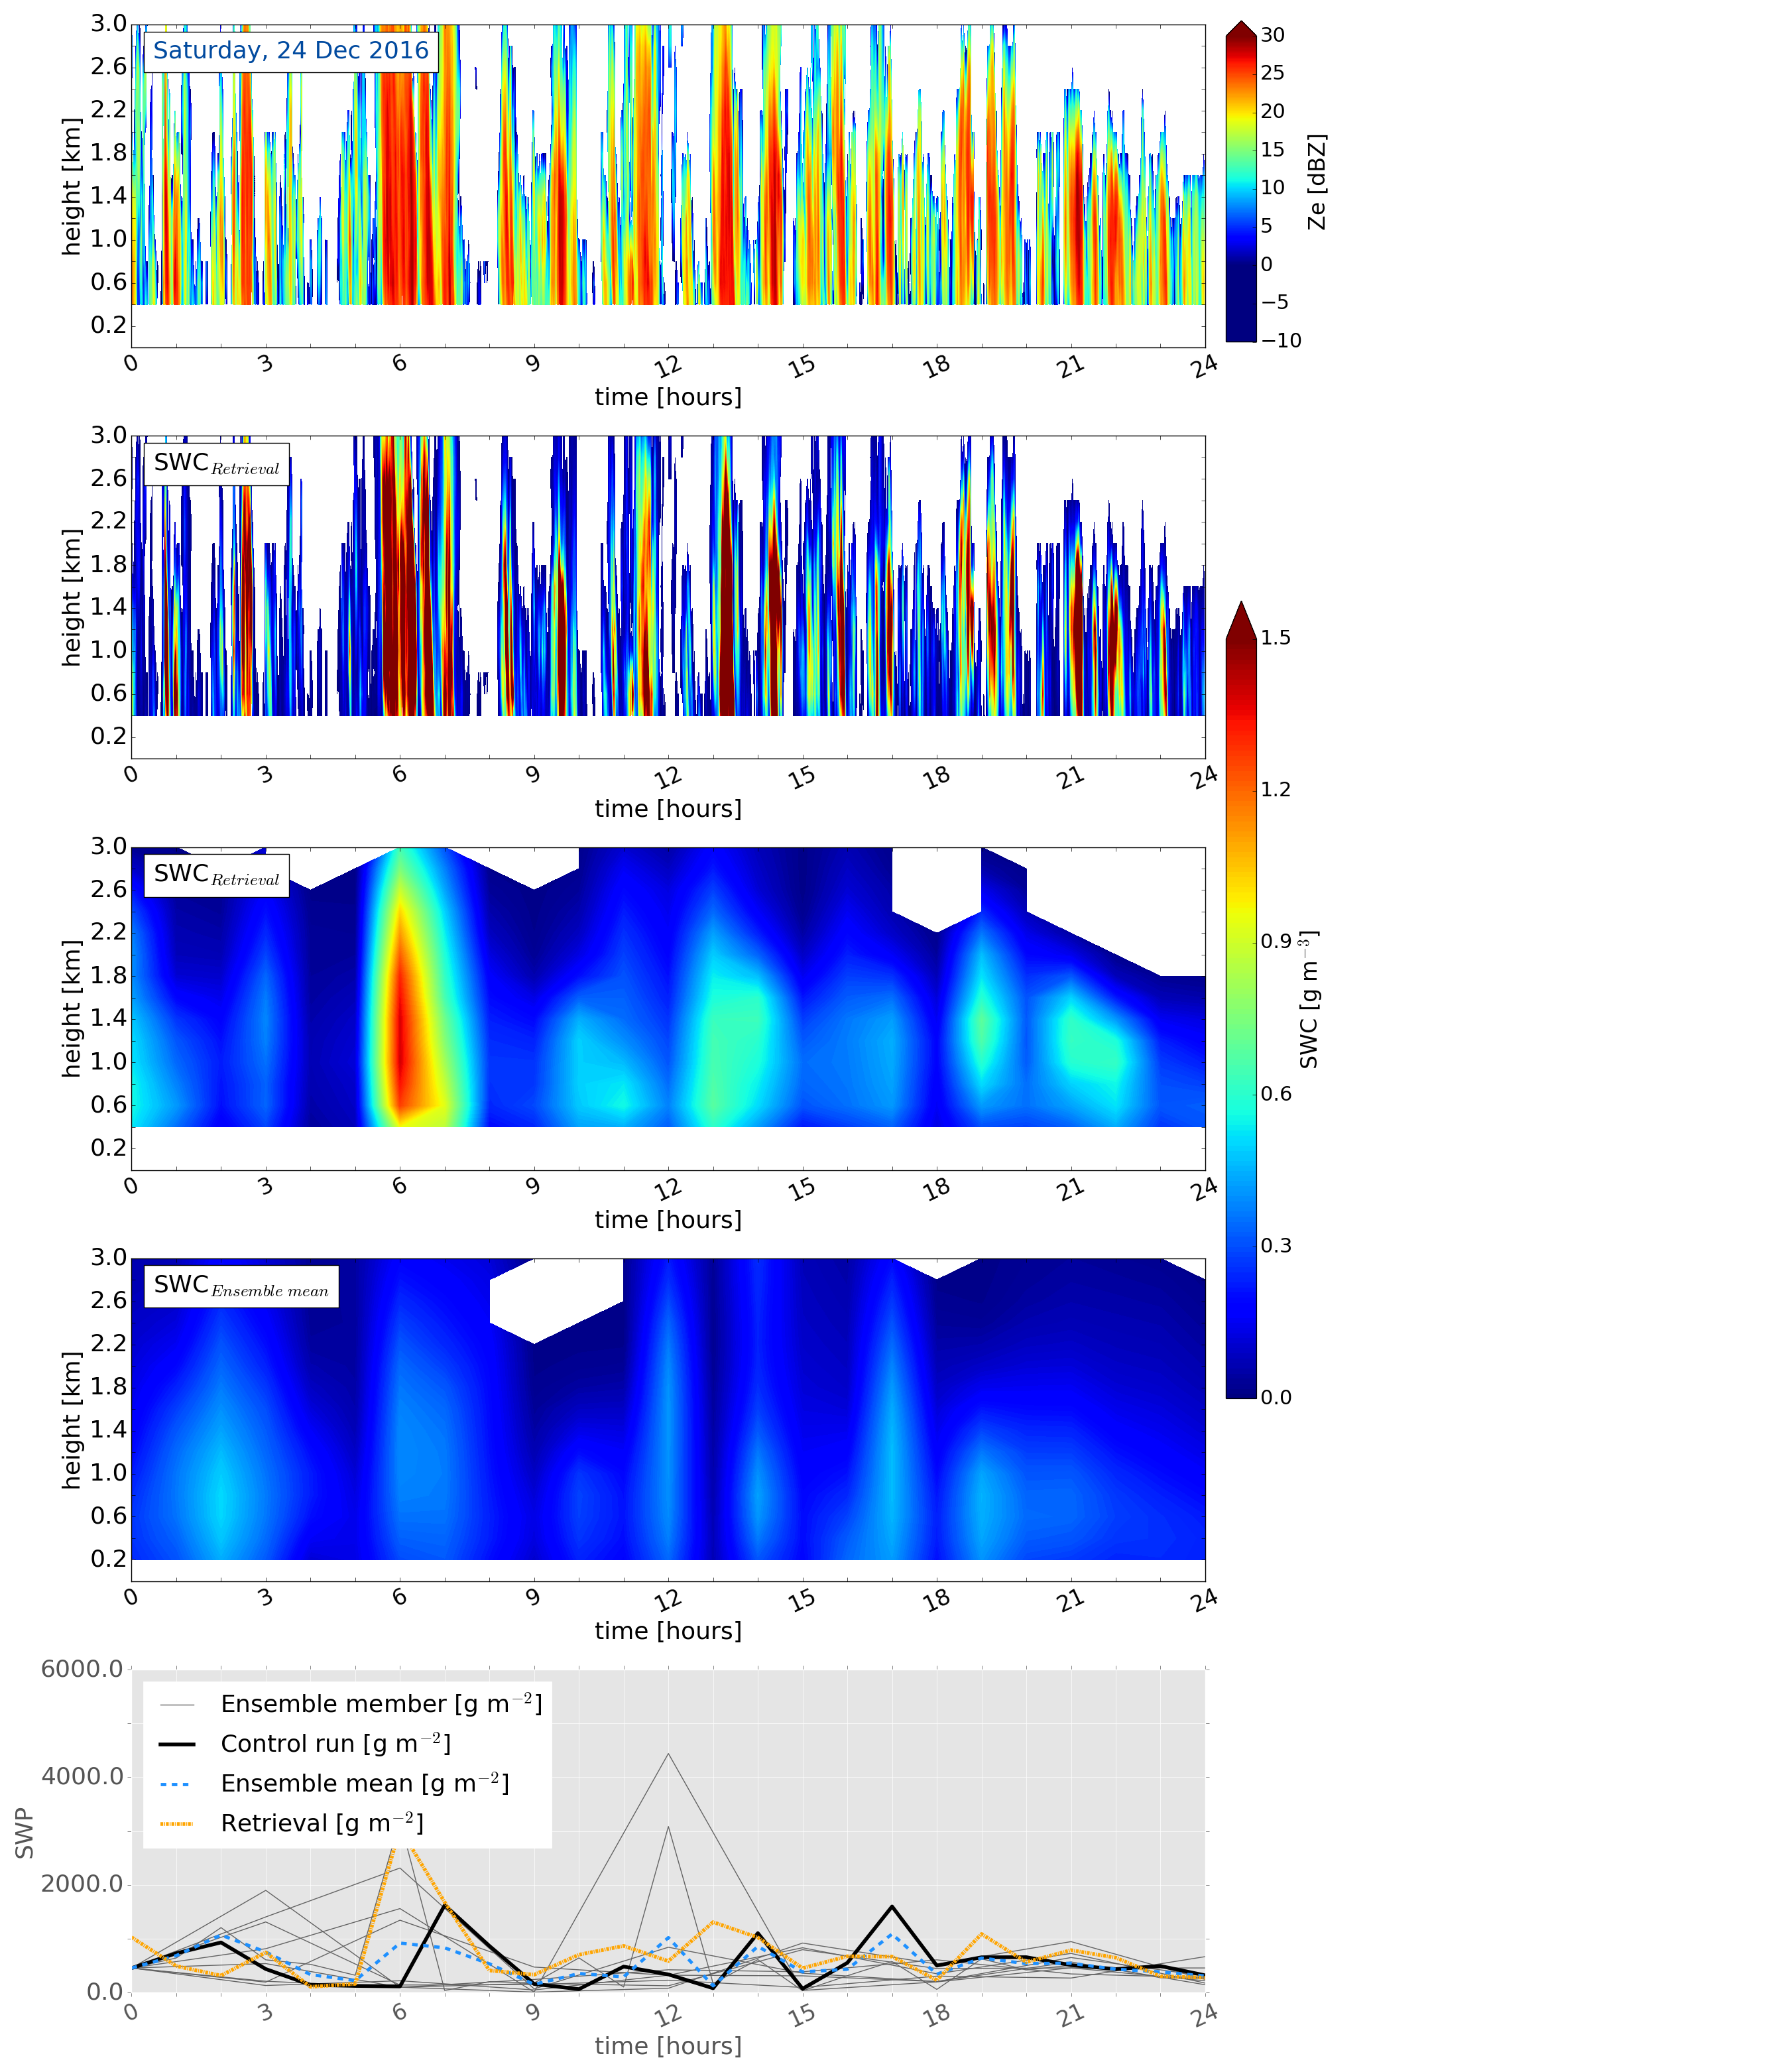
\includegraphics[trim={0.5cm 0.5cm 17.5cm .5cm},clip,width=\textwidth]{./fig_SWC/20161224}
	\caption{Saturday, \SI{21}{\dec}}\label{fig:SWC24}
\end{figure}
%%%%%%%%%%%%%%%%%%%%%%%%%%%%%%%%%%%%%%%%%%%%%%%%%%%%%%%%%%%%%%%%%%%%%%%%%%
%
% %%% image sounding MEPS %%%%%%%%%%%%%%%%%%%%%%%%%%%%%%%%%%%%%
% % !TeX spellcheck = en_GB
\begin{figure}
	\centering
	\begin{subfigure}[b]{0.49\textwidth}
		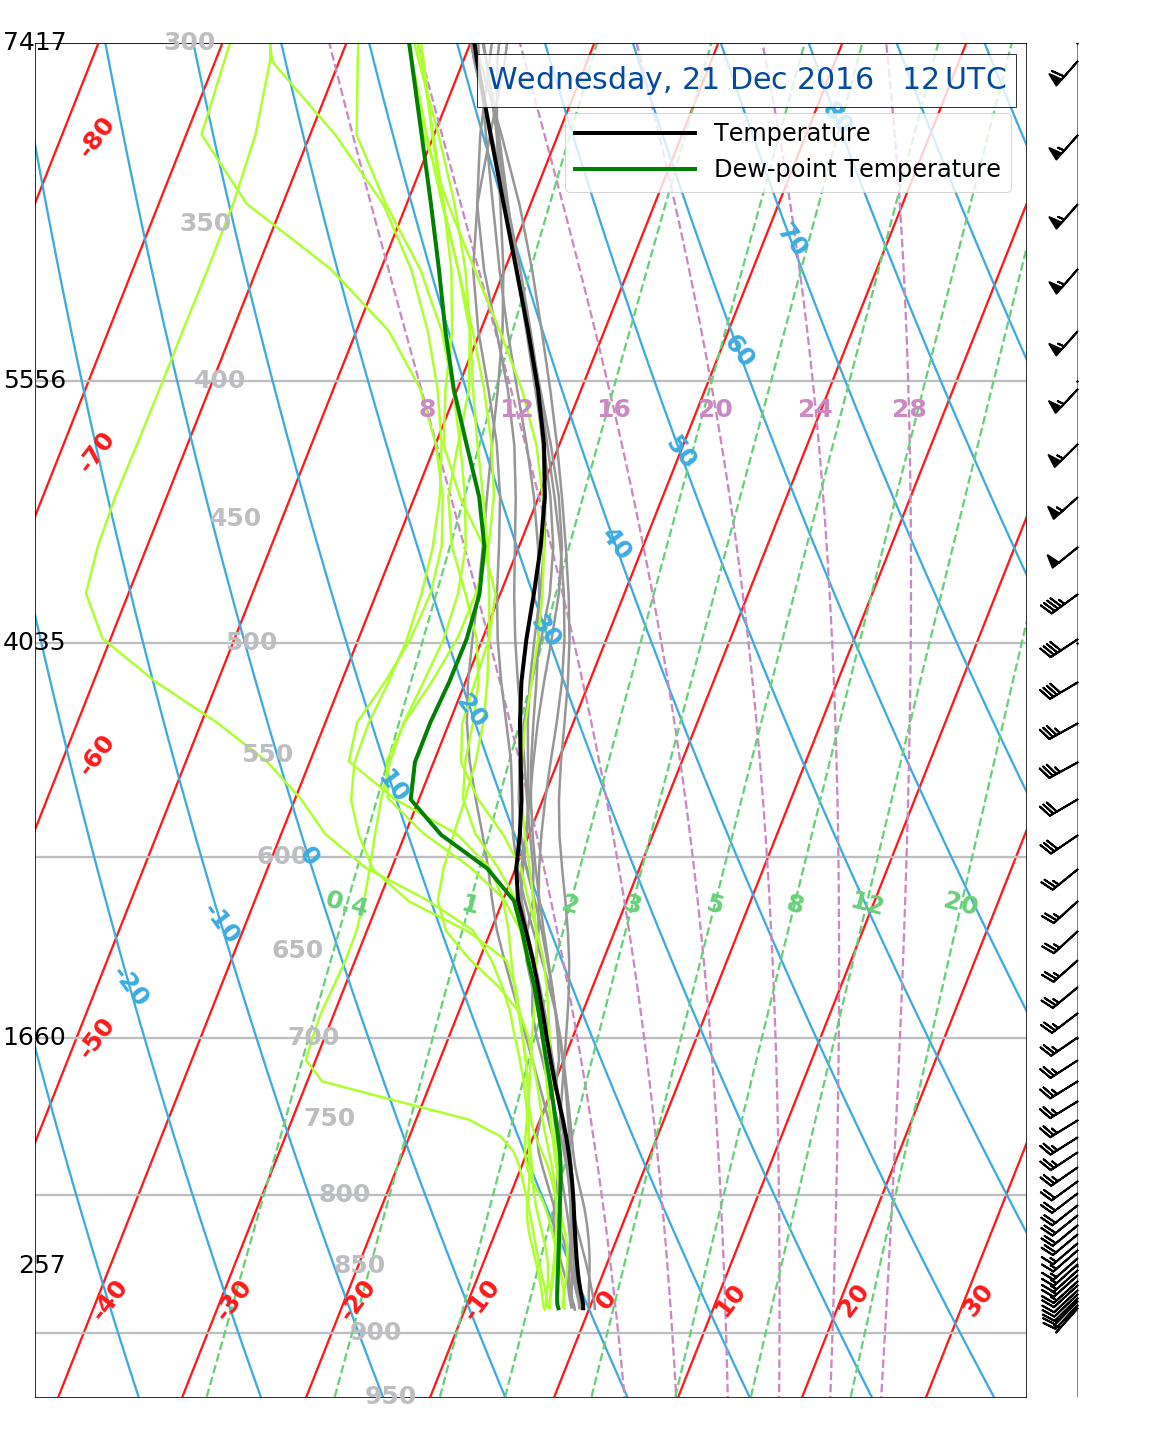
\includegraphics[width=\textwidth]{./fig_Sounding/20161220_36}
		\caption{}\label{fig:meps_sound_20}
	\end{subfigure}
	\begin{subfigure}[b]{0.49\textwidth}
		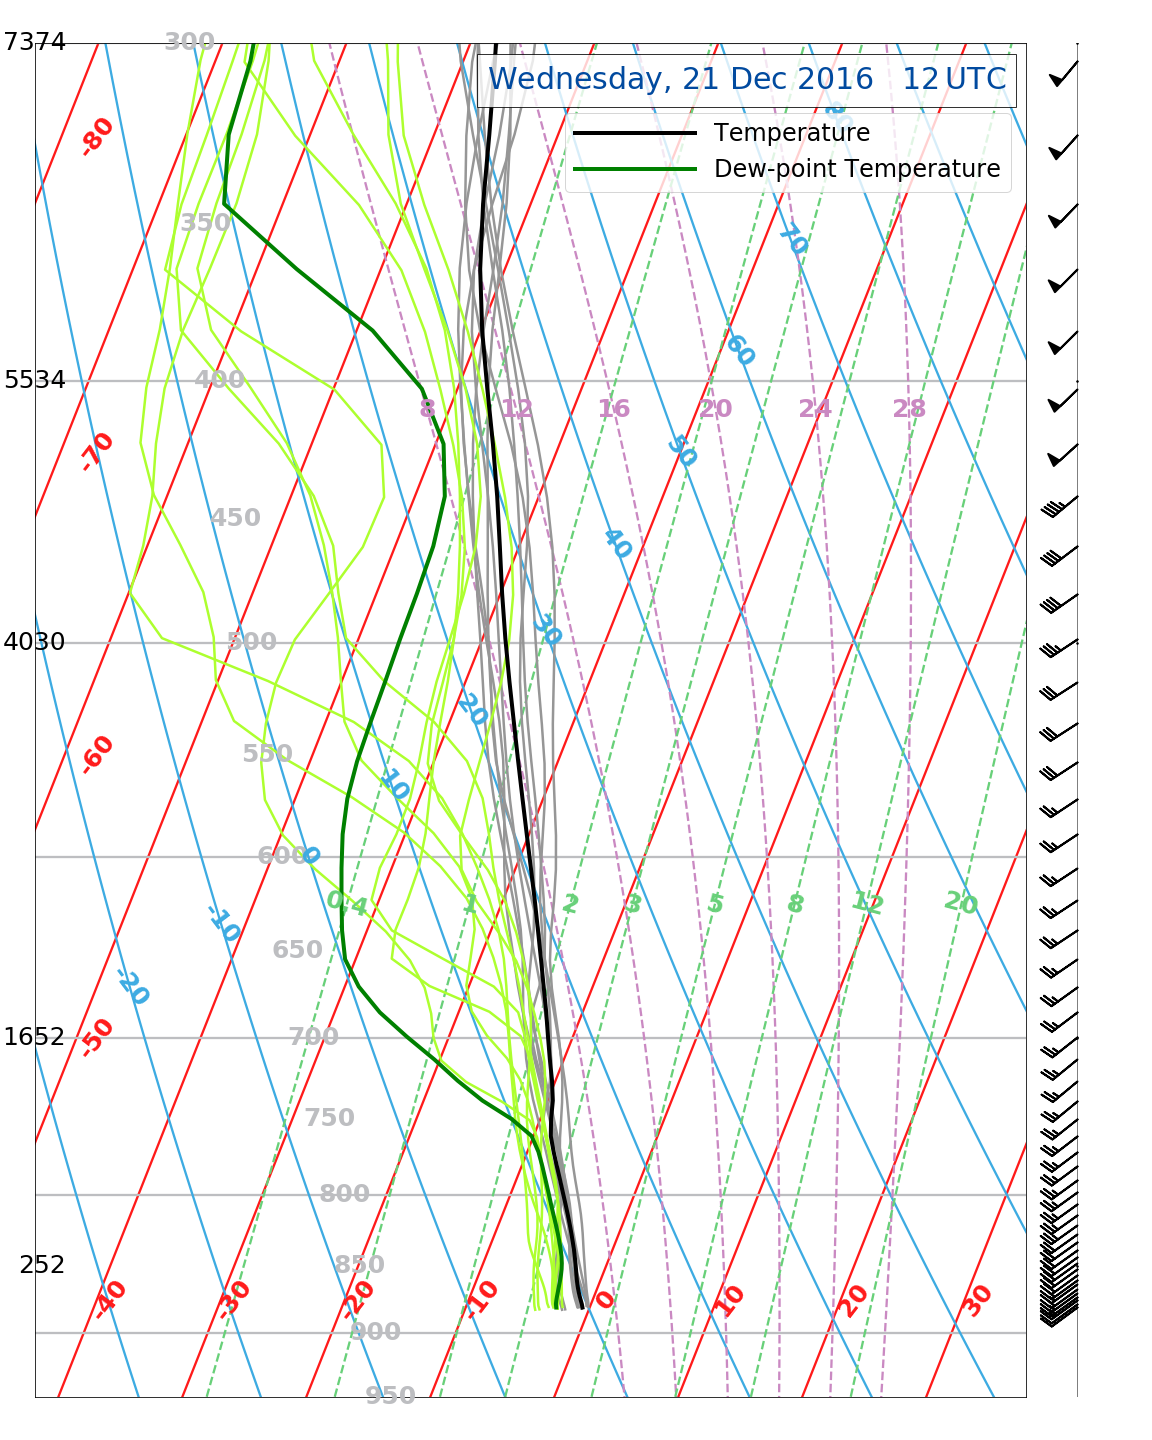
\includegraphics[width=\textwidth]{./fig_Sounding/20161221_12}
		\caption{}\label{fig:meps_sound_21}
	\end{subfigure}
	\caption{Vertical temperature profiles produced with MEPS. \protect{\subref{fig:meps_sound_20}} is initialised: Tuesday, \SI{20}{\dec} \SI{00}{\UTC}. \protect{\subref{fig:meps_sound_21}} is initialised: Wednesday, \SI{21}{\dec} \SI{00}{\UTC}.}
\end{figure}
% %%%%%%%%%%%%%%%%%%%%%%%%%%%%%%%%%%%%%%%%%%%%%%%%%%%%%%%%%%%%%%%%%%%%%%%%%%
% %

% %%% image ensemble spread %%%%%%%%%%%%%%%%%%%%%%%%%%%%%%%%%%%%%
\begin{figure}[h]
	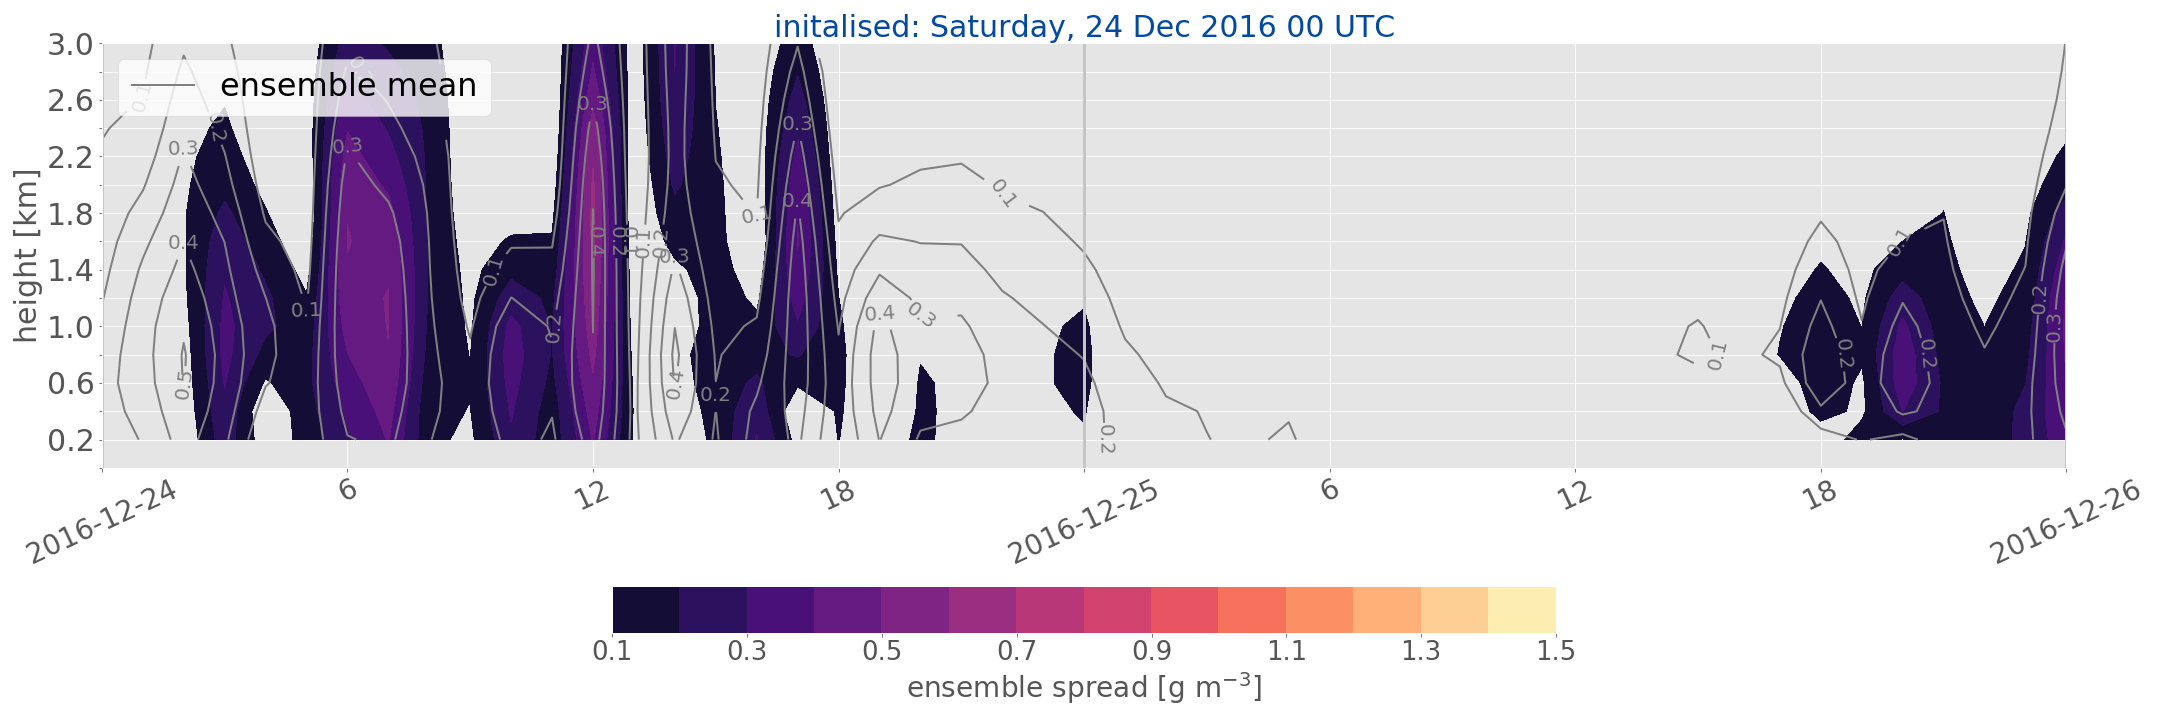
\includegraphics[width=\textwidth]{./fig_ensemble_spread/20161224}
	\caption{Ensemble spread indicated by the colour bar. Lighter colours show higher spread and darker colour very small spread of the ensemble members. Grey lines show the ensemble mean of the ten forecast members.}\label{fig:spread24}
\end{figure}
%
%%%%%%%%%%%%%%%%%%%%%%%%%%%%%%%%%%%%%%%%%%%%%%%%%%%%%%%%%%%%%%%%%%%%%%%%%%
%%%%%%%%% surface obs %%%%%%%%%%%%%%
\subsection{Surface accumulation}
%%% image surface accumulation %%%%%%%%%%%%%%%%%%%%%%%%%%%%%%%%%%%%%
\begin{figure}[h]
	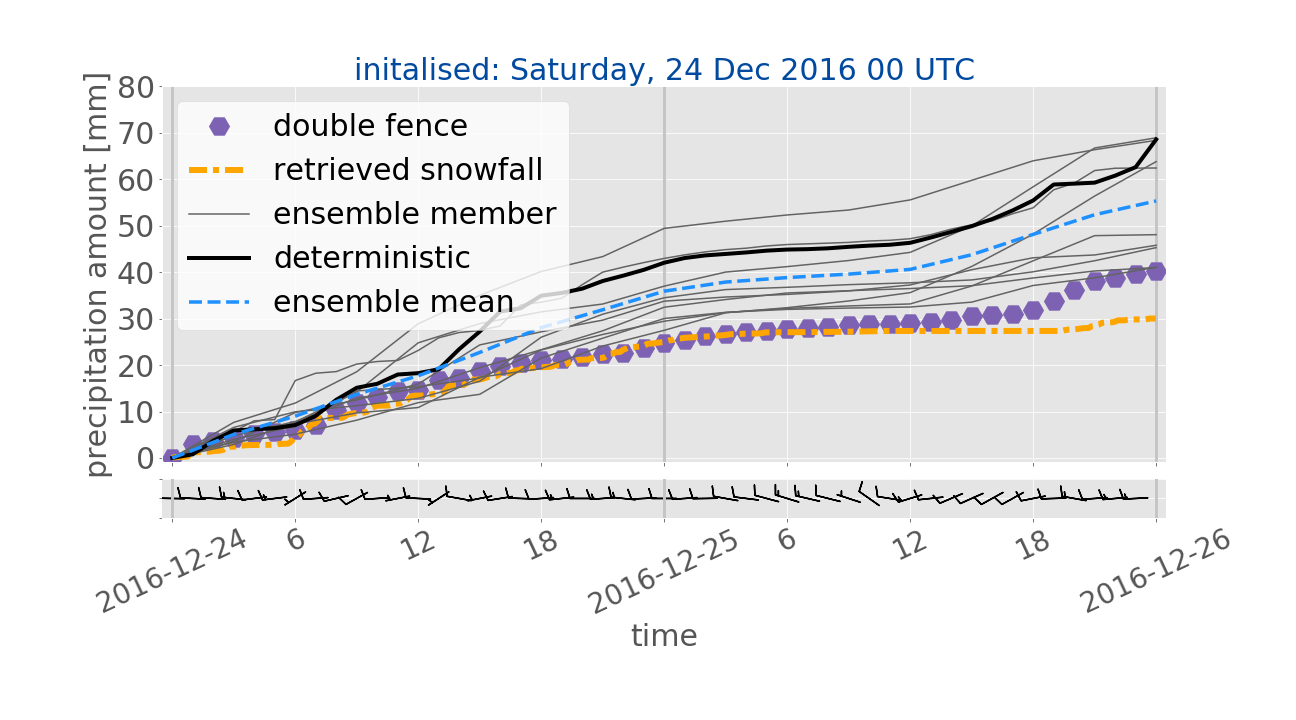
\includegraphics[width=\textwidth]{./fig_sfc_acc/acc_wind_20161224_00}
	\caption{}\label{fig:sfc_acc24}
\end{figure}
%%%%%%%%%%%%%%%%%%%%%%%%%%%%%%%%%%%%%%%%%%%%%%%%%%%%%%%%%%%%%%%%%%%%%%%%%%

%%% image surface MEPS boxplot %%%%%%%%%%%%%%%%%%%%%%%%%%%%%%%%%%%%%
\begin{figure}[h]
	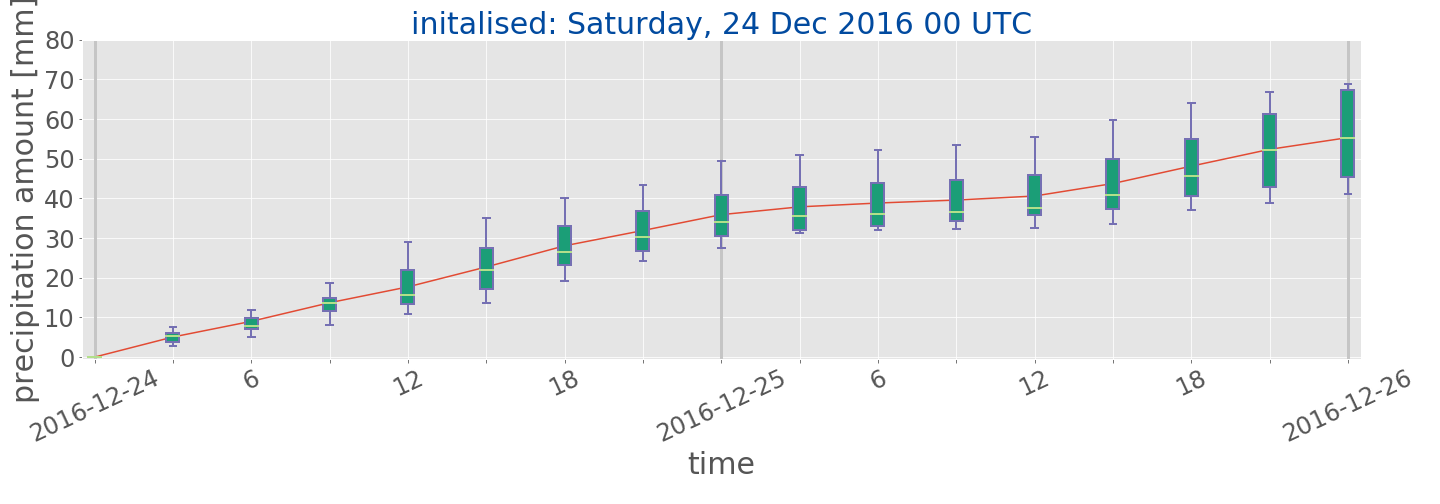
\includegraphics[width=\textwidth]{./fig_boxplot_sfc/20161224_0}
	\caption{Box-whisker-plot of the ten ensemble members of MEPS. Red line indicating the ensemble mean, lower and upper whisker the 25th and 75th percentile, respectively. Light green shows the median of all members and the box represents the middle \SI{50}{\percent} of scores of the precipitation.}\label{fig:boxplt24}
\end{figure}
%%%%%%%%%%%%%%%%%%%%%%%%%%%%%%%%%%%%%%%%%%%%%%%%%%%%%%%%%%%%%%%%%%%%%%%%%%
The box-whisker-plot in \Cref{fig:boxplt24} shows an uncertainty shortly after initialisation of the ten forecast members. All members have a different opinion of the precipitation amount, since the difference between the \SIrange{25}{75}{\percent} is wide spread.
The ensemble mean is always higher than the median and already after \SI{12}{\hour} forecast time is the median closer to the lower percentile. Also, all upper whiskers are taller than the lower ones, which would follow that the ensemble members vary amongst the most positive quartile and that it is very similar for the least positive quartile group.
\\
\textcolor{red}{DISCUSSION! The uncertainty shortly after the initialisation time might be associated with the spin up time of the precipitation value in the model. }

% %%% image surface MEPS wind scatter %%%%%%%%%%%%%%%%%%%%%%%%%%%%%%%%%%%%%
% \begin{figure}[h]
% %	\centering
%     \begin{subfigure}[b]{0.84\textwidth}
% 		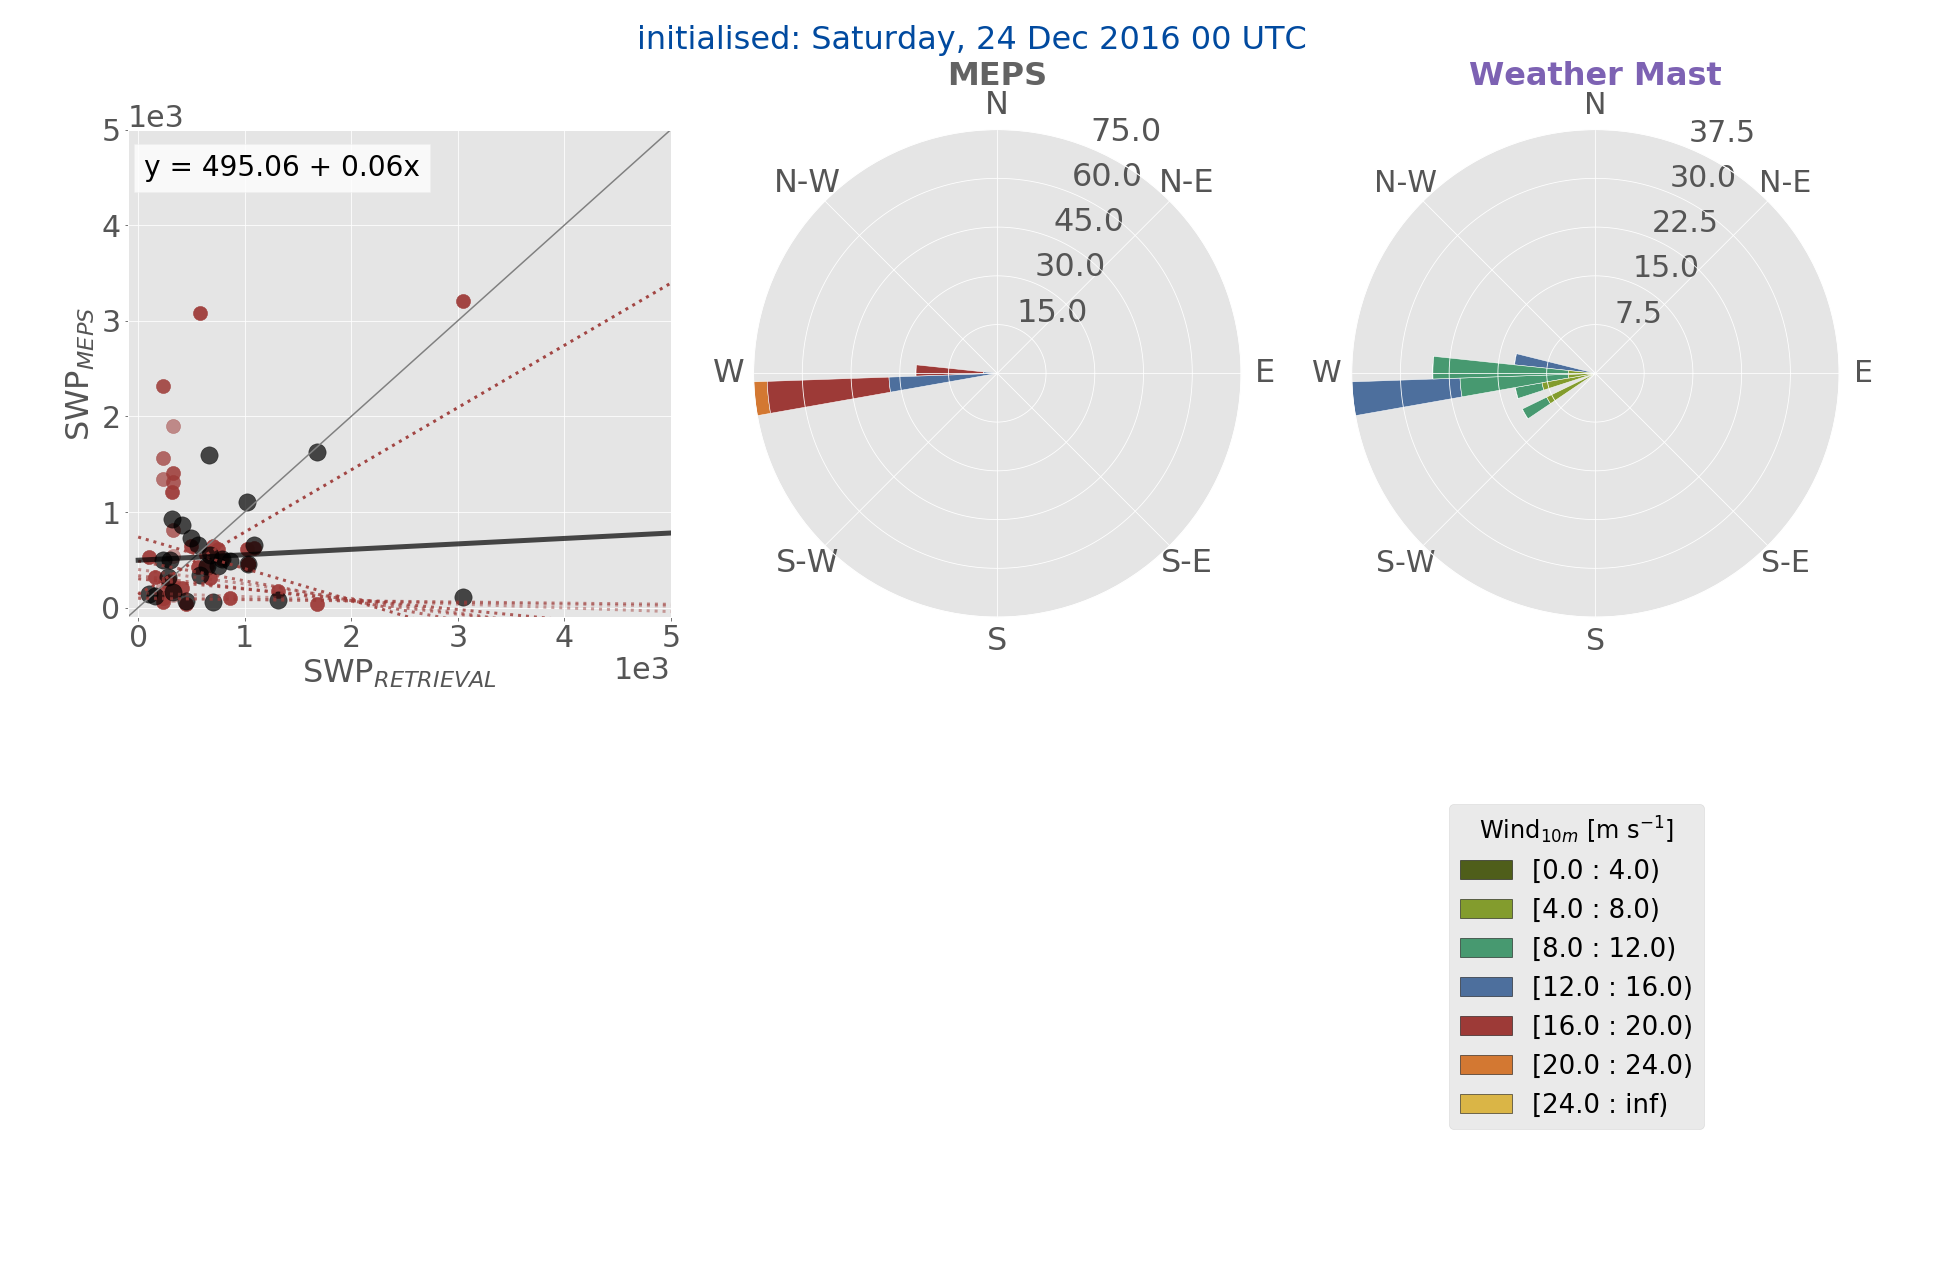
\includegraphics[trim={2.3cm 19.5cm 2.cm .7cm},clip,width=\textwidth]{./fig_windrose/20161224}
%     \end{subfigure}
% 	\begin{subfigure}[b]{0.15\textwidth}
% 		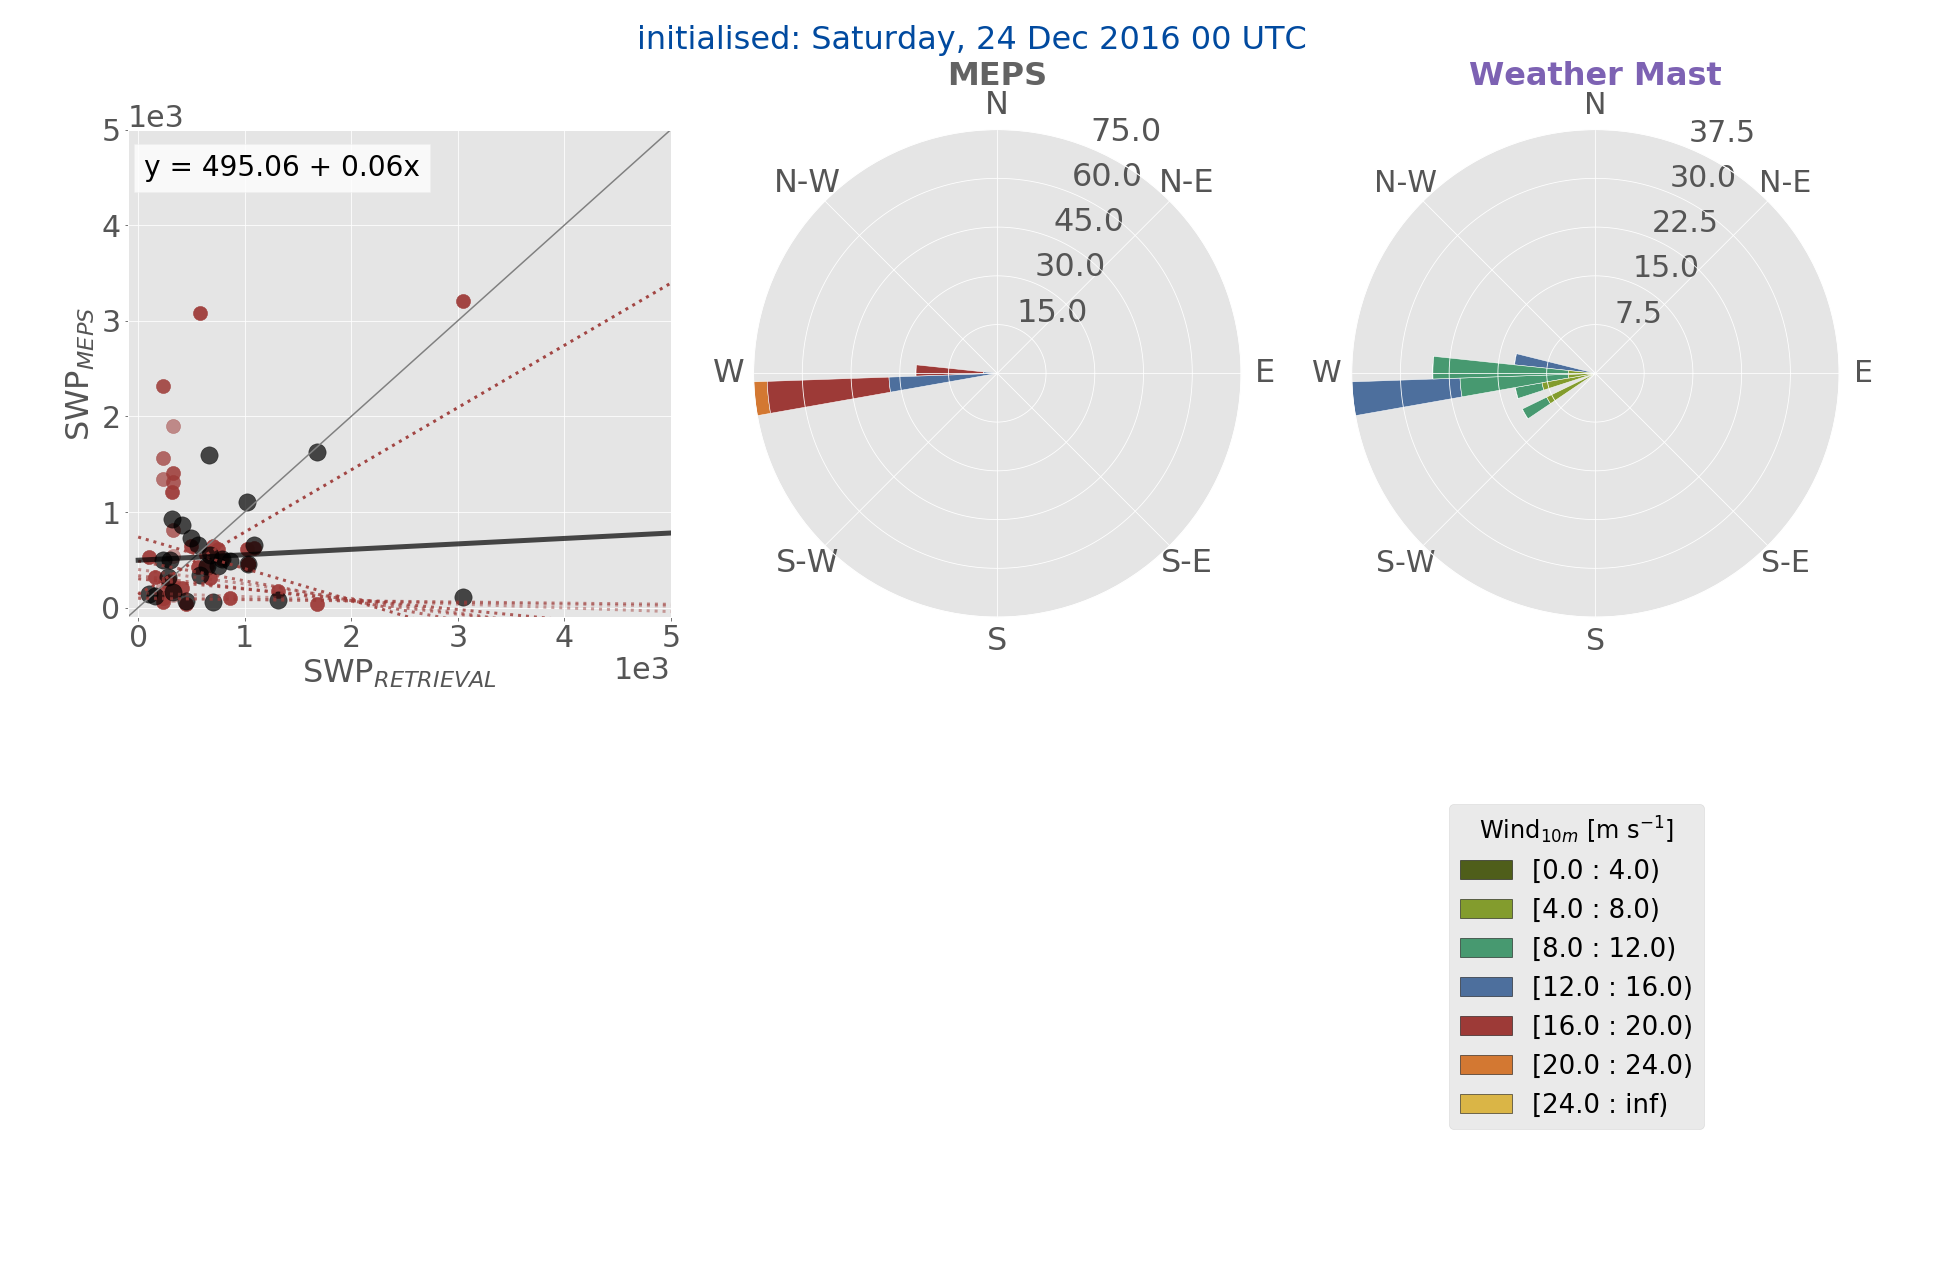
\includegraphics[trim={50.cm 0.cm 8.3cm 28.4cm},clip,width=\textwidth]{./fig_windrose/20161224}
% 	\end{subfigure}
%     \caption{}\label{fig:wind24}
% \end{figure}
% %%%%%%%%%%%%%%%%%%%%%%%%%%%%%%%%%%%%%%%%%%%%%%%%%%%%%%%%%%%%%%%%%%%%%%%%%%

%%%%%%%%%%%%%%%%%%%%%%%%%%%%%%%%%%%%%%%%%%%%%%%%%%%%%%%%%%%%%%%%%%%%%%%%%%























